\section[Euclidean Geometry]{Plane Euclidean Geometry}

\say{Candidates demonstrate an understanding of the foundations of geometry as outlined in the California Common Core Content Standards for Mathematics (Grade 7, Grade 8, and High School). Candidates demonstrate a depth and breadth of conceptual knowledge to ensure a rigorous view of geometry and its underlying structures. They demonstrate an understanding of \textbf{axiomatic systems} and different forms of \textbf{logical arguments}. Candidates understand, apply, and \textbf{prove theorems} relating to a variety of topics in \textbf{two- and three-dimensional geometry}, including \textbf{coordinate}, \textbf{synthetic}, \textbf{non-Euclidean}, and \textbf{transformational geometry}.}

\subsection{Parallel Postulate}

\textit{Apply the \textbf{Parallel Postulate} and its \textbf{implications} and justify its \textbf{equivalents} (e.g., the Alternate Interior Angle Theorem, the angle sum of every triangle is 180 degrees)}

\subsubsection*{Parallel Postulate}

\say{If a 
\href{https://en.wikipedia.org/wiki/Line_segment}{line segment} 
intersects two straight 
\href{https://en.wikipedia.org/wiki/Line_(geometry)}{lines} 
forming two interior angles on the same side that are less than two 
\href{https://en.wikipedia.org/wiki/Right_angle}{right angles}, 
then the two lines, if extended indefinitely, meet on that side on which the angles sum to less than two right angles.}
\href{https://en.wikipedia.org/wiki/Parallel_postulate}{Wikipedia}

\subsubsection*{implications}

The \textit{Parallel Postulate} is Euclid's 5th postulate:

\vspace{.25cm}
\say{And that if a straight-line falling across two (other) straight-lines makes internal angles on the same side(of itself whose sum is) less than two right-angles, then the two (other) straight-lines, being produced to infinity, meet on that side (of the original straight-line) that the(sum of the internal angles) is less than two right-angles (and do not meet on the other side}
\vspace{.25cm}



The following is based on this \href{https://search.brave.com/search?q=implications+of+the+parallel+postulate&source=desktop&summary=1&summary_og=eyJ0aXRsZSI6IkltcGxpY2F0aW9ucyBvZiB0aGUgcGFyYWxsZWwgcG9zdHVsYXRlIiwiZGVzY3JpcHRpb24iOiJUaGUgcGFyYWxsZWwgcG9zdHVsYXRlLCBhbHNvIGtub3duIGFzIEV1Y2xpZCdzIGZpZnRoIHBvc3R1bGF0ZSwgaGFzIGZhci1yZWFjaGluZyBpbXBsaWNhdGlvbnMgaW4gdmFyaW91cyBicmFuY2hlcyBvZiBtYXRoZW1hdGljcyBhbmQgc2NpZW5jZS4gSGVyZSBhcmUgc29tZSBvZiB0aGUga2V5IGltcGxpY2F0aW9uczpcblxuIE5vbi1FdWNsaWRlYW4gZ2Vv4oCmIiwiaW1hZ2UiOnsic3JjIjoiaHR0cHM6Ly9jZG4uc2VhcmNoLmJyYXZlLmNvbS9zZXJwL29nL2NlNmY1M2JkZTQ4YTYyODRkZjU5Y2IucG5nIiwid2lkdGgiOjQ4NCwiaGVpZ2h0Ijo1MDF9fQ%3D%3D&sig=3ef39a71b8d57bb4ab1a081ea832fe525929e28fc83d2e6e695ea40d80c6bdcc&nonce=00428446225450c7059fac239d7a9e3d}{AI generated answer}. 

\begin{enumerate}
    \item Non-Euclidian Geometries
    \item Reimannian geometry
    \item General relativity
    \item Toplology
    \item Computer Science
    \item Philosophy
    \item Mathematical Rigor
\end{enumerate}

\subsubsection*{equivalents}

The following is based on this \href{https://search.brave.com/search?q=equivalents+of+the+parallel+postulate&source=web&summary=1&summary_og=eyJ0aXRsZSI6IkVxdWl2YWxlbnRzIG9mIHRoZSBwYXJhbGxlbCBwb3N0dWxhdGUiLCJkZXNjcmlwdGlvbiI6IlRoZSBwYXJhbGxlbCBwb3N0dWxhdGUsIGFsc28ga25vd24gYXMgRXVjbGlkJ3MgZmlmdGggcG9zdHVsYXRlLCBoYXMgc2V2ZXJhbCBlcXVpdmFsZW50cyBpbiBnZW9tZXRyeS4gVGhlc2UgZXF1aXZhbGVudHMgYXJlIHN0YXRlbWVudHMgdGhhdCBjYW4gYmUgdXNlZCB0byByZXBsYWNlIHRoZSBwYXJhbGxlbCBwb3N0dWxhdGUgaW4gZ2VvbWV0cmljIHBy4oCmIiwiaW1hZ2UiOnsic3JjIjoiaHR0cHM6Ly9jZG4uc2VhcmNoLmJyYXZlLmNvbS9zZXJwL29nL2FmYzRiZDI2ZGYzYTgxOGVhNDc5YzIucG5nIiwid2lkdGgiOjQ4NCwiaGVpZ2h0Ijo1MDF9fQ%3D%3D&sig=6f2db1009466c13d483c3cfb5b7e103a48893164bb2702e696e38d9676c20e96&nonce=9a5bb06f7d55425d9ace01f4d630445e}{AI generated answer}. 




\subsection{Angles}

\textit{Demonstrate knowledge of \textbf{complementary}, \textbf{supplementary}, and \textbf{vertical} angles.}

\vspace{.25cm}

\say{In Euclidean geometry, an angle is the figure formed by two rays, called the sides of the angle, sharing a common endpoint, called the vertex of the angle.}\href{https://en.wikipedia.org/wiki/Angle}{Wikipedia}



\paragraph*{complementary angles}

The sum of two \textbf{complementary} angles is $90^\circ$.

\begin{figure}[h!]
    \centering
    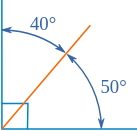
\includegraphics[width=2cm]{./public/images/complementary}
    \caption[short]{complementary angles}
\end{figure}

\say{The adjective complementary is from the Latin complementum, associated with the verb complere, "to fill up". An acute angle is "filled up" by its complement to form a right angle.}

\paragraph{supplementary angles}add up to $ 180^\circ$.

\begin{figure}[h!]
    \centering
    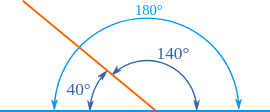
\includegraphics[width=4cm]{./public/images/supplementary}
    \caption[short]{supplementary angles}
\end{figure}

\paragraph*{vertical angles}

\href{https://en.wikipedia.org/wiki/Angle#Vertical_and_adjacent_angle_pairs}{vertical angles}are formed by two intersecting lines.
\subsection{Similarity and Congruence}


\textit{Prove theorems, justify steps, and solve problems involving \textbf{similarity} and \textbf{congruence}.}

\vspace{.5cm}



\subsubsection[similarity]{Similarity} 

Geometric similarity is a relation between two objects. Objects that have the same \textbf{shape} are said to be similar.

\paragraph*{triangle similarity} 

Triangles are similar if:all their angles are equal and corresponding sides are in the same ratio. There are three ways to find if two triangles are similar: 

AA, SAS and SSS:

\begin{description}
    \item[AA] AA stands for "angle, angle" and means that the triangles have two of their angles equal.
    \item[SAS] SAS stands for "side, angle, side" and means that we have two triangles where the ratio between two sides is the same as the ratio between another two sides and we we also know the included angles are equal. 
    \item[SSS] SSS stands for "side, side, side" and means that we have two triangles with all three pairs of corresponding sides in the same ratio. 
\end{description}

\subsubsection*{Similar Triangle Theorems}


The following are several properties of similar triangles. 

\paragraph*{Side-splitter Theorem}
This theorem is about lines that split a triangle into proportional side lengths.
\begin{figure}[h!]
    \centering
    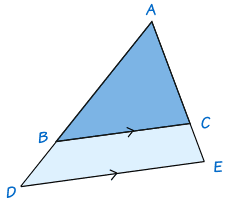
\includegraphics[width=2cm]{./public/images/side-splitter-theorem}
    \caption[side-splitter]{$BC \parallel DE \implies \frac{AB}{BD} = \frac{AC}{CE}$}
\end{figure}

\paragraph*{Angle Bisector Theorem}
This theorem is about proportional sides and angle bisectors.
\begin{figure}[h!]
    \centering
    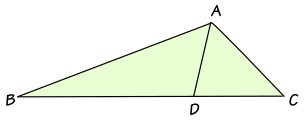
\includegraphics[width=3cm]{./public/images/angle-bisector-theorem}
    \caption[side-splitter]{$\overline{AD}  bisects \angle BAC \implies \frac{AB}{BD} = \frac{AC}{DC}$}
\end{figure}

\subsubsection[Congruence]{Congruence} 

There are five ways to find if two triangles are congruent: SSS, SAS, ASA, AAS and HL.\footnote{\href{https://www.mathsisfun.com/geometry/triangles-congruent-finding.html}{math is fun}}

\subsubsection[short]{side, side, side(SSS)}

SSS stands for "side, side, side" and means that we have two triangles with all three sides equal.

\begin{figure}[h!]
    \centering
    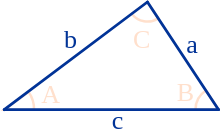
\includegraphics[width=4cm]{./public/images/sss}
    \caption[SSS]{side, side, side}
\end{figure}

The \textbf{Law of Cosines} can be used to find angles.
\subsection{properties of triangles}

\textit{Apply and justify properties of triangles (e.g., the \textbf{Exterior Angle Theorem}, \textbf{concurrence theorems}, \textbf{trigonometric ratios}, \textbf{triangle inequality}, \textbf{Law of Sines}, \textbf{Law of Cosines}, the \textbf{Pythagorean Theorem} and its \textbf{converse})}

\subsubsection{Exterior Angle Theorem}

\begin{figure}[h!]
    \centering
    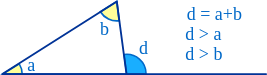
\includegraphics[width=4cm]{./public/images/exterior-angle-theorem}
    \caption[exterior-angle]{exterior angle theorem}
\end{figure}

\vspace{4cm}

\subsubsection{concurrence theorems}

\begin{figure}[h!]
    \centering
    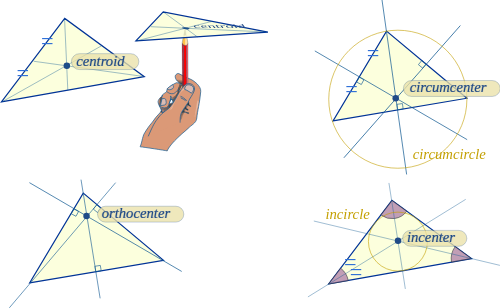
\includegraphics[width=8cm]{./public/images/triangle-centers}
    \caption{triangle centers}
\end{figure}

\paragraph*{centroid} Draw a line (called a "median") from each corner to the midpoint of the opposite side.
Where all three lines intersect is the centroid, which is also the "center of mass":

\begin{figure}[h!]
    \centering
    \begin{subfigure}{2cm}
        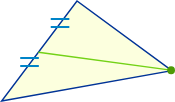
\includegraphics[width=2cm]{./public/images/median}
        \caption{median}
    \end{subfigure}
    \begin{subfigure}{3cm}
        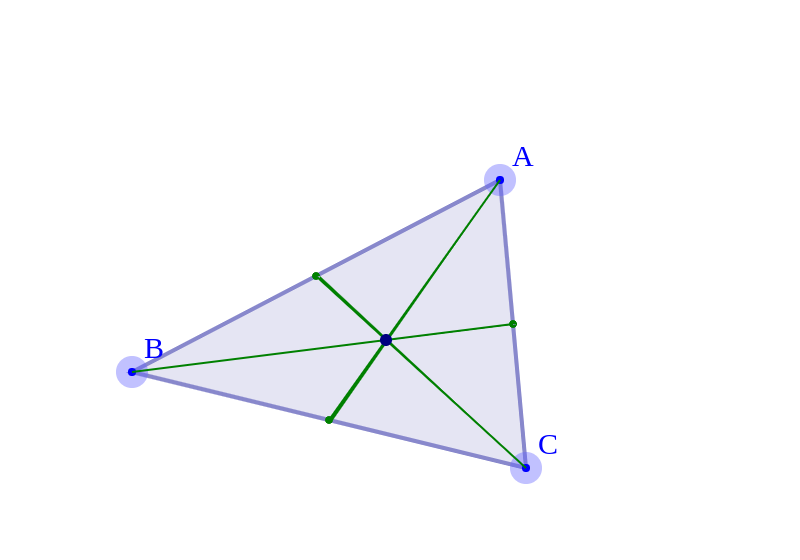
\includegraphics[width=3cm]{./public/images/centroid}
        \caption{centroid}
    \end{subfigure}
    \caption{median $\implies$ centroid}
\end{figure}

\paragraph*{circumcenter} Draw a line (called a "perpendicular bisector") at right angles to the midpoint of each side.Where all three lines intersect is the center of a triangle's "circumcircle", called the "circumcenter":

\begin{figure}[h!]
    \centering
    \begin{subfigure}{3cm}
        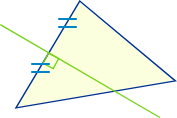
\includegraphics[width=2.5cm]{./public/images/perpendicular-bisector}
        \caption{perpendicular bisector}
    \end{subfigure}
    \begin{subfigure}{3cm}
        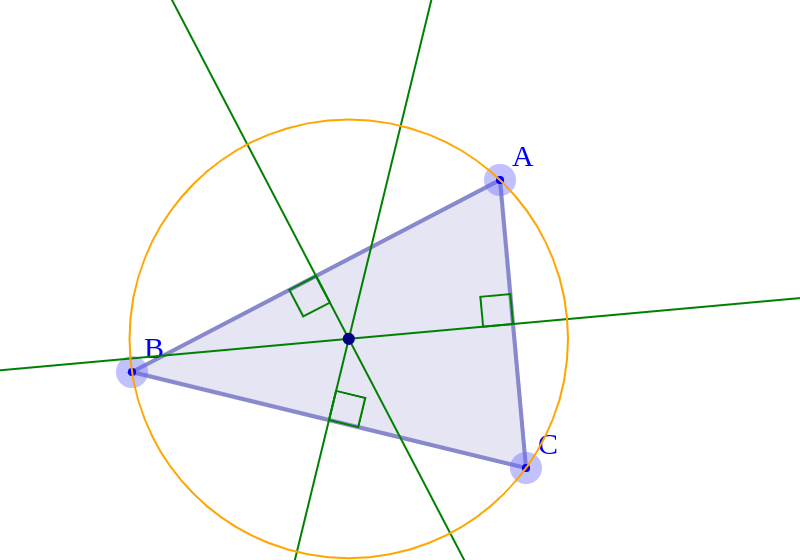
\includegraphics[width=3cm]{./public/images/circumcenter}
        \caption{circumcenter}
    \end{subfigure}
    \caption{perpendicular bisector $\implies$ circumcenter}
\end{figure}


\paragraph*{incenter} Draw a line (called the "angle bisector") from a corner so that it splits the angle in half
Where all three lines intersect is the center of a triangle's "incircle", called the "incenter":

\begin{figure}[h!]
    \centering
    \begin{subfigure}{3cm}
        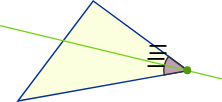
\includegraphics[width=2.5cm]{./public/images/angle-bisector}
        \caption{angle bisector}
    \end{subfigure}
    \begin{subfigure}{3cm}
        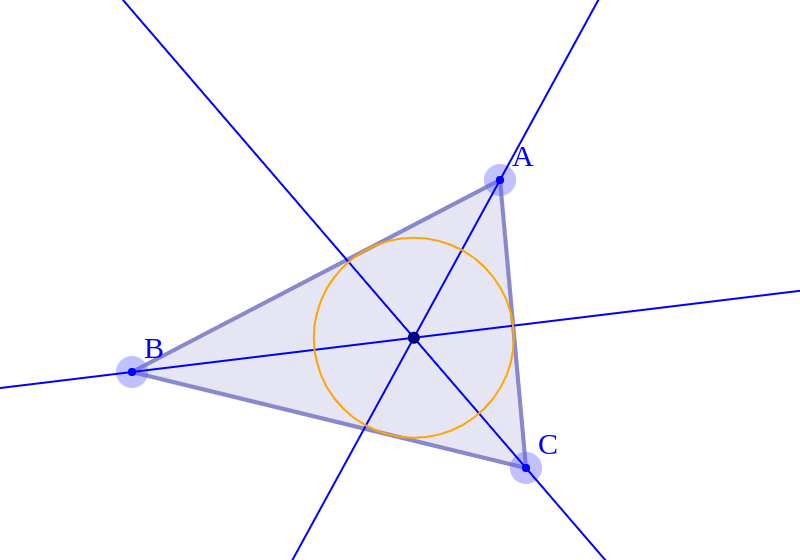
\includegraphics[width=3cm]{./public/images/incenter}
        \caption{incenter}
    \end{subfigure}
    \caption{angle bisector $\implies$ incenter}
\end{figure}
\subsubsection{trigonometric ratios} 

\subsubsection{triangle inequality}

\subsubsection{Law of Sines}

\subsubsection{Law of Cosines}

\subsubsection{Pythagorean Theorem}

\subsubsection{Pythagorean Theorem (converse)}
\subsection{polygons and circles}

\textit{Apply and justify properties of polygons and circles from an advanced standpoint (e.g.,
derive the area formulas for regular polygons and circles from the area of a triangle)}

\subsection{classical constructions}

\textit{Identify and justify the classical constructions (e.g., angle bisector, perpendicular bisector,
replicating shapes, regular polygons with 3, 4, 5, 6, and 8 sides)}



\footnote[1]{(California Common Core Content Standards for Mathematics, including Standards for Mathematical Practice
1–8: Geometry, Grade 7 [7.G]; Geometry, Grade 8; Congruence, High School [G-CO]; Similarity, Right
Triangles, and Trigonometry, High School [G-SRT]; Circles, High School [G-C]; Geometric Measurement and
Dimension, High School [G-GMD])}